% How hard each piece of the Lab Standard is to ignore: asks < shows < blocks.
% Colours come from src/styles/palette.json via the generated ../_palette.tex (npm run tokens).
% Shared house style for the TikZ diagrams. render.sh defines \theme (light|dark) before \input.
\documentclass{article}
\usepackage{fontspec}
\usepackage{tikz}
\usepackage{fontawesome5}
\usetikzlibrary{positioning,calc,arrows.meta,fit,backgrounds}
\setmainfont{CrimsonPro}[Path=\fontdir, Extension=.ttf, UprightFont=*, ItalicFont=*-Italic, UprightFeatures={RawFeature={+wght=400}}, ItalicFeatures={RawFeature={+wght=400}}, BoldFont=*, BoldFeatures={RawFeature={+wght=600}}, Scale=1.08]
\setmonofont{JetBrainsMono}[Path=\fontdir, Extension=.ttf, Scale=0.86]
\newfontfamily\kickerfont{JetBrainsMono}[Path=\fontdir, Extension=.ttf, Scale=0.72, LetterSpace=12]
% GENERATED from src/styles/palette.json by scripts/tokens/build.mjs. Do not edit; run `npm run tokens`.
\def\darktheme{dark}
\ifx\theme\darktheme
  \definecolor{ink}{HTML}{EFEFE8}
  \definecolor{muted}{HTML}{A0A09A}
  \definecolor{paper}{HTML}{1B1B19}
  \definecolor{accent}{HTML}{5FE08F}
  \definecolor{accentfill}{HTML}{173322}
  \definecolor{oxide}{HTML}{FF6A4D}
\else
  \definecolor{ink}{HTML}{111111}
  \definecolor{muted}{HTML}{4A4A4A}
  \definecolor{paper}{HTML}{FFFFF8}
  \definecolor{accent}{HTML}{1F7A45}
  \definecolor{accentfill}{HTML}{E6F1EA}
  \definecolor{oxide}{HTML}{C8361C}
\fi

\tikzset{
  every picture/.style={line cap=round, line join=round, font=\normalsize, text=ink},
  card/.style={draw=ink!70!paper, line width=0.6pt, fill=paper, rounded corners=3pt, align=left,
               text width=#1, inner xsep=7pt, inner ysep=5.5pt, anchor=north west},
  card/.default=3.9cm,
  hot/.style={card=#1, draw=accent, line width=1.1pt, fill=accentfill},
  hot/.default=3.9cm,
  ghost/.style={card=#1, draw=muted!80!paper, dashed, fill=none, text=muted},
  ghost/.default=3.9cm,
  panel/.style={draw=muted!45!paper, line width=0.5pt, rounded corners=5pt, inner sep=9pt},
  hotpanel/.style={panel, draw=accent!75!paper, line width=0.9pt},
  line/.style={-{Stealth[length=5pt,width=4.2pt]}, line width=0.7pt, draw=ink!70!paper},
  hotline/.style={line, draw=accent, line width=1pt},
  ghostline/.style={line, draw=muted!80!paper, dashed},
  badline/.style={line, draw=oxide, line width=1pt},
  lbl/.style={font=\small\itshape, text=muted, inner sep=2.5pt},
  head/.style={font=\itshape, text=muted, anchor=south west, inner sep=0pt, align=left},
  warm/.style={card=#1, draw=accent!60!paper, fill=accentfill!50!paper},
  warm/.default=3.9cm,
}
\newcommand{\kicker}[1]{{\kickerfont\MakeUppercase{#1}}}
\newcommand{\ico}[1]{\makebox[1.25em][l]{#1}}
\newcommand{\cardtext}[2]{{\ttfamily #1}\\[1pt]{\small\itshape\color{muted}#2}}
% Crop the page to the picture: typeset it into a box and ship that box as the page.
\newcommand{\diagram}[1]{%
  \setbox0\hbox{#1}%
  \pagewidth=\dimexpr\wd0+8pt\relax \pageheight=\dimexpr\ht0+\dp0+8pt\relax
  \hoffset=-1in \voffset=-1in
  \shipout\vbox{\kern4pt\hbox{\kern4pt\box0}}}

\begin{document}
\diagram{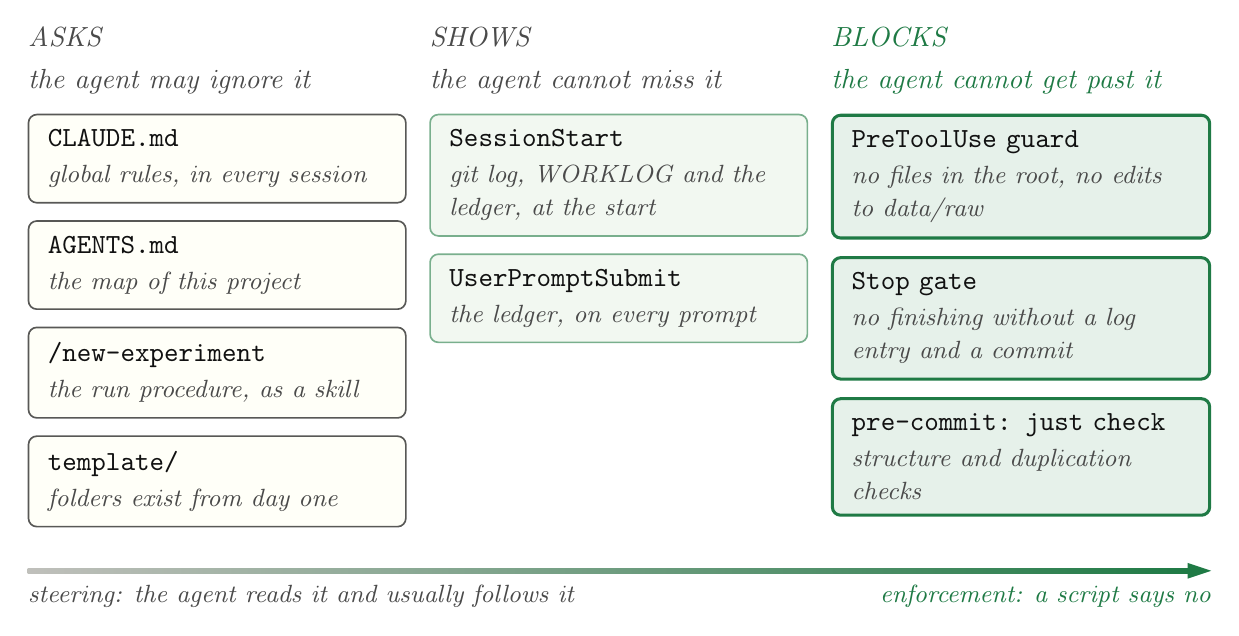
\begin{tikzpicture}[x=1cm,y=1cm]
  \def\w{4.3cm}
  % column heads
  \node[head] at (0,0.25)   {\kicker{asks}\\[3pt] the agent may ignore it};
  \node[head] at (5.1,0.25) {\kicker{shows}\\[3pt] the agent cannot miss it};
  \node[head, text=accent] at (10.2,0.25) {\kicker{blocks}\\[3pt] the agent cannot get past it};
  % asks
  \node[card=\w] (a1) at (0,0) {\cardtext{CLAUDE.md}{global rules, in every session}};
  \node[card=\w, below=6pt of a1.south west, anchor=north west] (a2) {\cardtext{AGENTS.md}{the map of this project}};
  \node[card=\w, below=6pt of a2.south west, anchor=north west] (a3) {\cardtext{/new-experiment}{the run procedure, as a skill}};
  \node[card=\w, below=6pt of a3.south west, anchor=north west] (a4) {\cardtext{template/}{folders exist from day one}};
  % shows
  \node[warm=\w] (s1) at (5.1,0) {\cardtext{SessionStart}{git log, WORKLOG and the ledger, at the start}};
  \node[warm=\w, below=6pt of s1.south west, anchor=north west] (s2) {\cardtext{UserPromptSubmit}{the ledger, on every prompt}};
  % blocks
  \node[hot=\w] (b1) at (10.2,0) {\cardtext{PreToolUse guard}{no files in the root, no edits to data/raw}};
  \node[hot=\w, below=6pt of b1.south west, anchor=north west] (b2) {\cardtext{Stop gate}{no finishing without a log entry and a commit}};
  \node[hot=\w, below=6pt of b2.south west, anchor=north west] (b3) {\cardtext{pre-commit: just check}{structure and duplication checks}};
  % the axis underneath: how binding each layer is
  \coordinate (L) at ($(a4.south west)+(0,-0.55)$);
  \coordinate (R) at ($(L -| b3.east)$);
  \shade[left color=muted!35!paper, right color=accent, draw=none]
    ($(L)+(0,-0.03)$) rectangle ($(R)+(-0.25,0.03)$);
  \fill[accent] ($(R)+(-0.3,0.1)$) -- (R) -- ($(R)+(-0.3,-0.1)$) -- cycle;
  \node[font=\small\itshape, text=muted, anchor=north west, inner sep=0pt] at ($(L)+(0,-0.18)$) {steering: the agent reads it and usually follows it};
  \node[font=\small\itshape, text=accent, anchor=north east, inner sep=0pt] at ($(R)+(0,-0.18)$) {enforcement: a script says no};
\end{tikzpicture}}
\end{document}
